\documentclass{beamer}

%%% Fonts
\usepackage[T1]{fontenc}
% \usepackage{roboto}
\usepackage[scaled]{helvet}

\usepackage{emoji}

\setbeamertemplate{footline}[frame number]
\setbeamertemplate{headline}{}
\setbeamertemplate{navigation symbols}{}

\usefonttheme[onlymath]{serif}
\setbeamerfont{normal text}{family=\sffamily,size*={12pt}{14pt},series=\mdseries}
\setbeamerfont{alerted text}{parent=normal text}

\setbeamerfont{structure}{parent=normal text,series=\mdseries}

\setbeamerfont{footline}{parent=structure,size*={8pt}{10pt}}

\setbeamerfont{title}{size*={14pt}{16pt},parent=alerted text,shape=\scshape}
\setbeamerfont{title in head/foot}{parent=footline,series=\bfseries}

\setbeamerfont{subtitle}{parent=title,shape=\upshape}

\setbeamerfont{section in toc}{parent=normal text}
\setbeamerfont{subsection in toc}{parent=section in toc}
\setbeamerfont{subsubsection in toc}{parent=subsection in toc}

\setbeamerfont{author}{parent=normal text}
\setbeamerfont{author in head/foot}{parent=footline}
\setbeamerfont*{institute}{parent=normal text}

\setbeamerfont{frametitle}{parent=alerted text,size*={16pt}{18pt}}
\setbeamerfont{caption}{series=\normalfont, size=\small}
\setbeamerfont{caption name}{series=\normalfont, size=\small}

\setbeamerfont*{itemize/enumerate body}{parent=normal text}
\setbeamerfont*{itemize/enumerate subbody}{parent=itemize/enumerate body}
\setbeamerfont*{itemize/enumerate subsubbody}{parent=itemize/enumerate subbody}
%%%

\usepackage[vlined]{algorithm2e}
\usepackage{booktabs}
\usepackage{annotate-equations}
\usepackage{pgfplots}
\usepackage{tikz}
\usepackage[style=alphabetic]{biblatex}

\bibliography{references}

\definecolor{NavyBlue}{HTML}{2280ff}
\definecolor{orange}{HTML}{E69F00}
\definecolor{skyblue}{HTML}{56B4E9}
\definecolor{bluishgreen}{HTML}{009E73}
\definecolor{yellow}{HTML}{F0E442}
\definecolor{blue}{HTML}{0072B2}
\definecolor{vermilion}{HTML}{D55E00}
\definecolor{reddishpurple}{HTML}{CC79A7}
\definecolor{black}{HTML}{000000}

\pgfplotsset{compat=1.18}
% \usepgfplotslibrary{external}
% \tikzexternalize

\renewcommand*{\thefootnote}{\fnsymbol{footnote}}

\DeclareMathOperator*{\argmax}{arg\,max}
\DeclareMathOperator*{\argmin}{arg\,min}
\renewcommand{\epsilon}{\varepsilon}
% \newcommand{\Cset}{\mathcal{C}_S}
\newcommand{\Let}[2]{#1 $\leftarrow$ #2}
\newcommand{\proxy}[1]{\pi\left(#1\right)}
\newcommand{\assign}[1]{\phi\left(#1\right)}
\newcommand{\wassign}[1]{\hat{\phi}\left(#1\right)}
\newcommand{\assignprime}[1]{\phi'\left(#1\right)}
\newcommand{\optassign}[1]{\phi^\star\left(#1\right)}
\newcommand{\nearest}[1]{\operatorname{nrst}\left(#1\right)}
\newcommand{\optf}{\ensuremath{OPT_{fair}}}
\newcommand{\optu}{\ensuremath{OPT_{unf}}}


\title{Coresets for Fair $k$-center clustering}
\author{\emph{Matteo Ceccarello}}
\institute{U. of Padova}
\date{Joint work with Andrea Pietracaprina and Geppino Pucci}

\begin{document}

\frame{\titlepage}

% \begin{frame}{Outline}
% 	\begin{itemize}
% 		\item Problem definition
% 		\item Related work
% 		\item A LP solution
% 		\item Sequential coreset construction
% 		\item MapReduce coreset construction
% 		\item Streaming coreset construction
% 		\item Conclusions
% 	\end{itemize}
%
% \end{frame}



\begin{frame}{Problem definition}
	\centering

	\only<1>{
		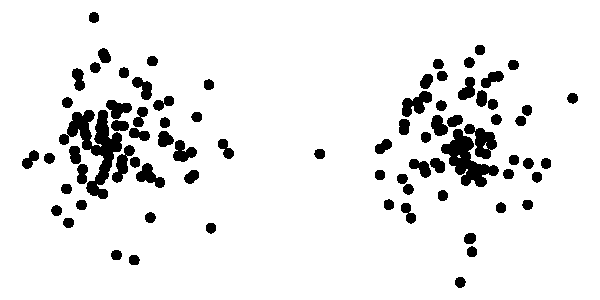
\includegraphics[width=\textwidth]{figs/example-no-color.pdf}
	}
	\only<2>{
		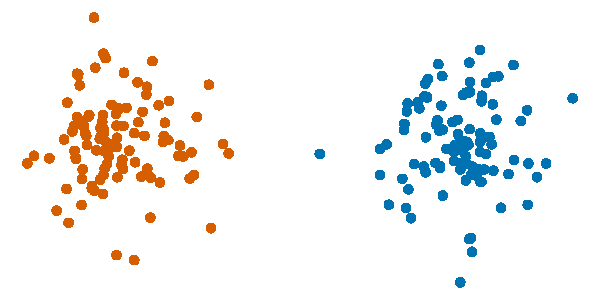
\includegraphics[width=\textwidth]{figs/example-color.pdf}
	}
	\only<3>{
		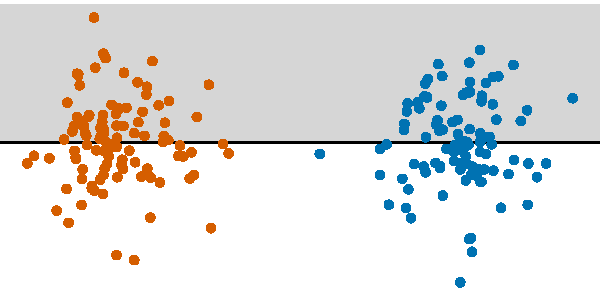
\includegraphics[width=\textwidth]{figs/example-color-clustering.pdf}
	}

\end{frame}



\begin{frame}{Problem definition}
	\begin{block}{Disparate impact}
		Protected attributes (e.g. gender, ethnicity\dots) should
		not be used directly to make decisions, and people in different protected
		classes should not experience disproportionally different outcomes.
	\end{block}

	\pause

	\begin{block}{Unawareness does not help}
		Blindly ignoring protected attributes
		is no solution: correlated features (e.g. height which correlates with
		sex) can leak information about the protected attributes and thus lead to
		\emph{unfair} solutions.
	\end{block}
\end{frame}





\begin{frame}{Problem definition}
	\begin{block}{Goal}
		Build a clustering such that the \emph{proportion} of points from
		each protected group is the same as the proportion in the entire dataset.
	\end{block}

	\pause

	\begin{block}{Example}
		At a wedding party, half of the people are friends of one spouse,
		\alert{half} are friends of the other.
		Our clusters are the $k$ tables at which people will be sitting:
		we want to have,
		for each table,
		\alert{half} of the the people from each group,
		so they can become friends.
	\end{block}
	\pause
	\begin{center}
		\Large
		\emoji{heart}
	\end{center}
\end{frame}






\begin{frame}{Problem definition}
	\begin{itemize}
		\item Metric space $(\mathcal{X}, d)$
		\item Set of points $S$
		\item Each point has one (or more) colors out of a set $\Gamma$
		\item Parameter $k$
	\end{itemize}
\end{frame}





\begin{frame}{Problem definition}
	\begin{block}{Doubling dimension}
		In a metric space of doubling dimension $D$ a ball of radius $r$
		can be covered by $2^D$ balls of radius $r/2$.
	\end{block}
	\centering
	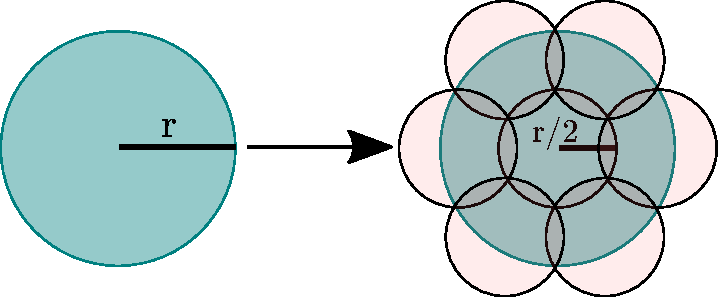
\includegraphics[width=\textwidth]{figs/doubling-dimension.pdf}
\end{frame}





\begin{frame}{Problem definition}
	\vfill

	\begin{equation*}
		r_{\eqnmarkbox[NavyBlue]{centers}{C}, \eqnmarkbox[vermilion]{assign}{\phi}}(S)
		= \max_{x \in \eqnmarkbox[skyblue]{input}{S}}
		\eqnmarkbox[reddishpurple]{distance}{d}(x, \eqnmarkbox[orange]{assignment}{\phi(x)})
	\end{equation*}

	\annotate[yshift=2em]{above,left}{distance}{distance function}
	\annotate[yshift=1em]{above,left}{centers}{find set of centers $\subseteq S$}
	\annotate[yshift=-1em]{below,left}{assign}{find assignment $\phi: S \to C$}
	\annotate[yshift=-1em]{below,right}{input}{input set}
	\annotate[yshift=1em]{above}{assignment}{center of $x$}

	\pause

	\vspace{2em}
	Minimize the above, where the assignment is subject to
	\vspace{2em}

	\begin{equation*}
		\eqnmarkbox[orange]{beta}{\beta_\ell}
		\le
		\frac{
			\left|\{x \in S : \eqnmarkbox[orange]{colorcluster}{col(x) = \ell }
			\wedge
			\eqnmarkbox[NavyBlue]{assign1}{\phi(x) = c}
			\} \right|
		}{
			\left| \{ x \in S : \eqnmarkbox[NavyBlue]{assign2}{ \phi(x) = c} \} \right|
		}
		\le
		\eqnmarkbox[orange]{alpha}{\alpha_\ell}
		\quad
		\forall \eqnmarkbox[NavyBlue]{center}{c \in C},
		\eqnmarkbox[orange]{color}{ \ell \in \Gamma }
	\end{equation*}

	\annotate[yshift=1em]{above,right}{center}{cluster centers}
	\annotate[yshift=1em]{above,left}{colorcluster}{points with color $\ell$}
	\annotate[yshift=0.6em]{above}{assign1}{assigned to $c$}
	\annotate[yshift=-0.5em]{below}{assign2}{assigned to $c$}
	\annotate[yshift=-1em]{below,left}{color}{set of colors}
	\annotatetwo[yshift=-3.4em]{below}{beta}{alpha}{fairness constraints}

	\vfill

\end{frame}





\begin{frame}{Problem definition}
	\begin{block}{Additive violation}
		The additive violation of an assignment, w.r.t. the fairness constraints
		$\alpha_\ell, \beta_\ell$, is the minimum $\mathcal{E}$ s.t.
		$\forall c \in C, \ell \in \Gamma$
		\vspace{3em}
		\[
			\eqnmarkbox[vermilion]{c1}{\beta_\ell |\mathcal{C}_c|}
			\eqnmarkbox[NavyBlue]{v1}{- \mathcal{E}}
			\le
			{ |\mathcal{C}_{c, \ell}| }
			\le
			\eqnmarkbox[vermilion]{c2}{\alpha_\ell |\mathcal{C}_c|}
			\eqnmarkbox[NavyBlue]{v2}{+ \mathcal{E}}
		\]
	\end{block}
	\annotatetwo[yshift=1.4em]{above}{c1}{c2}{constraints on the number of points with color $\ell$ in $C$}
	\annotatetwo[yshift=-1.4em]{below}{v1}{v2}{violation}

	\vspace{2em}
	Where
	\[\mathcal{C}_c = \{x \in S : \phi(x) = c\}\]
	\[\mathcal{C}_{c, \ell} = \{x \in S : \phi(x) = c \wedge col(x) = \ell\}\]

\end{frame}





\begin{frame}{Problem definition}
	\begin{block}{Notation}
		\begin{itemize}
			\item $\optu$ cost of an \emph{unfair} optimal solution
			\item $\optf$ cost of an \emph{fair} optimal solution
		\end{itemize}
	\end{block}


	\pause

	\begin{block}{}
		\[
			\optu \le \optf
		\]
	\end{block}
\end{frame}











\begin{frame}{State of the art}

	\centering
	{\footnotesize
		\begin{tabular}{l r l c}
			\toprule
			                                        & approximation & violation & \# variables                              \\
			\midrule
			\cite{DBLP:conf/nips/Chierichetti0LV17} & 4             & --        & $\dagger$                                 \\
			% \cite{DBLP:conf/icalp/Rosner018}        & 14            & --        & $\dagger$                                 \\
			\cite{DBLP:conf/approx/Bercea0KKRS019}  & 5             & 0         & $O(n^2)$                                  \\
			                                        & 3             & $1$       & $O(n^2)$                                  \\
			\cite{DBLP:conf/nips/BeraCFN19}         & 4 (3)         & $7$       & $O(k\cdot n)$                             \\
			\cite{DBLP:conf/nips/HarbL20}           & 3             & $7$       & $O(\min\{k\cdot n, |\Gamma| 2^{k-1} k\})$ \\
			% \cite{DBLP:conf/www/BeraDGK22}          & 9 (MR)                   & 7         & $O(p \cdot k\cdot n)$                     \\
			%                                         & $7+\epsilon$ (streaming) & 7         & $O(p \cdot k\cdot n)$                     \\
			\bottomrule
		\end{tabular}
	}

	\footnotetext[2]{
		combinatorial solution
	}
\end{frame}
\begin{frame}{Our contribution}

	\centering
	{\footnotesize
		\begin{tabular}{l r l c}
			\toprule
			                                        & approximation                                   & violation & \# variables                                                                                                         \\
			\midrule
			\cite{DBLP:conf/nips/Chierichetti0LV17} & 4                                               & --        & $\dagger$                                                                                                            \\
			% \cite{DBLP:conf/icalp/Rosner018}        & 14            & --        & $\dagger$                                                              \\
			\cite{DBLP:conf/approx/Bercea0KKRS019}  & 5                                               & 0         & $O(n^2)$                                                                                                             \\
			                                        & 3                                               & $1$       & $O(n^2)$                                                                                                             \\
			\cite{DBLP:conf/nips/BeraCFN19}         & 4 (3)                                           & $7$       & $O(k\cdot n)$                                                                                                        \\
			\cite{DBLP:conf/nips/HarbL20}           & 3                                               & $7$       & $O(\min\{\qquad~~\qquad k\cdot n, |\Gamma| 2^{k-1} k\})$                                                             \\
			\midrule
			Our work                                & $\eqnmarkbox[NavyBlue]{contrib1}{ 3+\epsilon }$ & $7$       & $O(\min\{k\cdot \eqnmarkbox[NavyBlue]{contrib2}{ k|\Gamma|\left(\frac{c}{\epsilon}\right)^D }, |\Gamma|2^{k-1} k\})$ \\
			\bottomrule
		\end{tabular}
	}

	\annotatetwo[yshift=-2em]{below}{contrib1}{contrib2}{Our contribution}

	% \vspace{1em}
	% We provide MapReduce and Streaming algorithms as well.
\end{frame}












\begin{frame}{Preliminaries: GMM}
	\vfill
	Classic algorithm for \emph{unfair} $k$-center.
	\vfill

	\begin{algorithm}[H]
		\KwIn{Set $S$, parameter $k$}

		\BlankLine
		\Let{$C$}{$\{\textrm{arbitrary point from } S\}$}\;
		\While{$|C| < k$}{
			\Let{$c$}{$\argmax_{x\in S} d(x, C)$}\;
			\Let{$C$}{$C \cup \{c\}$}\;
		}
		\Return $C$\;
	\end{algorithm}

	\vfill
	Provides a 2-approximation in time $O(k\cdot n)$
	\vfill
\end{frame}






















\begin{frame}{Starting point~\cite{DBLP:conf/nips/BeraCFN19,DBLP:conf/nips/HarbL20}}
	\begin{block}{Algorithm}
		\begin{enumerate}
			\item Find a set $C$ of centers with the GMM algorithm
			\item Do a binary search on guesses over the possible clustering radii
			\item Instantiate a linear program and find a fractional solution (if any)
			\item If the linear program has a feasible solution,
			      then iteratively round it (will not see today).
		\end{enumerate}
	\end{block}

	\pause

	\begin{block}{Guarantees}
		\begin{itemize}
			\item The algorithm provides a $3$ approximation to the radius
			\item The fairness constraints have an additive violation up to $7$
		\end{itemize}
	\end{block}

\end{frame}








\begin{frame}{Starting point~\cite{DBLP:conf/nips/BeraCFN19}}
	\vfill

	Let $C$ be the set of $k$ centers found by GMM, and $R$ be a radius guess.

	\vspace{1em}

	\begin{align*}
		0 \le \eqnmarkbox[vermilion]{vardef}{z_{x, c}} \le & ~ 1
		\;                                                 &
		% \substack{ x \in S, c\in C                               \\ \textrm{if } d(x, c) \le R}
		\substack{ x \in S                                       \\ c\in C }  \textrm{ if } d(x, c) \le \eqnmarkbox[reddishpurple]{R}{R}
		\\
		\sum_{ c \in C } z_{x, c} =                        & ~ 1
		% \eqnmarkbox[skyblue]{onecluster}{1}
		\;                                                 &
		\forall x \in S
		\\
		% Fairness lower
		\beta_\ell \eqnmarkbox[bluishgreen]{fullcluster1}{ \sum_{x\in S} z_{x, c} }
		\le                                                &
		\eqnmarkbox[orange]{colorcluster}{\sum_{x'\in S_\ell} z_{x', c}}
		\le           \alpha_\ell
		\eqnmarkbox[bluishgreen]{fullcluster2}{\sum_{x\in S} z_{x, c}}
		\;                                                 &
		\forall c\in C, \ell\in\Gamma
	\end{align*}

	\annotate[yshift=1em]{above,left}{R}{Radius guess}
	\annotate[yshift=1em]{above, right}{vardef}{Is $x$ assigned to $c$?}
	% \annotate[yshift=.5em]{above, right}{onecluster}{Assign to only one cluster}
	\annotate[yshift=-.5em, xshift=0em]{below, right}{colorcluster}{Points of color\\ $\ell$ assigned to $c$}
	\annotatetwo[yshift=-3em]{below}{fullcluster1}{fullcluster2}{Size of cluster centered at $c$}

	\vfill

\end{frame}







% \begin{frame}{Coresets}
% 	% Let $(O_S, \phi_S)$ be an optimal $k$-center solution on $S$.
% 	% A pointset $T \subseteq S$ is a coreset if the cost
% 	% of an optimal solution $O_T\subseteq S$ has cost
% 	% \[
% 	% 	r_{O_T,\phi_T} \le
% 	% 	(1+\epsilon)
% 	% 	r_{O_S,\phi_S}
% 	% \]
% 	\begin{equation}
% 		r_{\eqnmarkbox[orange]{tsol}{C_T, \phi_T}}(T)
% 		\le (1 + \epsilon)
% 		r_{\eqnmarkbox[NavyBlue]{ssol}{C_S, \phi_S}}(S)
% 	\end{equation}
% \end{frame}






\begin{frame}{Outline of our approach}
	\begin{enumerate}
		\item Build a \emph{weighted} coreset $T$ out of the input set $S$
		\item Compute a fair $k$-center clustering on of $T$, whose centers are $C$
		\item Build a fair assignment of $S$ to $C$ by using information from the solution on the coreset
	\end{enumerate}

	\vfill\hrule\vfill
	\pause

	\begin{columns}
		\begin{column}[t]{0.49\textwidth}
			\centering
			In MapReduce, steps 1. and 3. are carried out in a single parallel round each
		\end{column}
		\begin{column}[t]{0.49\textwidth}
			\centering
			In Streaming, steps 1. and 3. require each a pass on the data
		\end{column}
	\end{columns}


\end{frame}








\begin{frame}{Sequential coreset construction}
	\begin{algorithm}[H]
		\KwIn{Set $S$, parameter $k$, parameter $\epsilon$}

		\BlankLine
		\Let{$T$}{$\{\textrm{arbitrary point from } S\}$}\;
		\lWhile{$|T| < k$}{
			\Let{$T$}{$T \cup \{  \argmax_{x\in S} d(x, T) \}$}
		}

		\pause
		\Let{$r_k$}{$\max_{x \in S} d(x, T)$}\;

		\pause
		\While{$\max_{x\in S} d(x, T) > \frac{\epsilon}{6}\cdot r_k$}{
			\Let{$T$}{$T \cup \{  \argmax_{x\in S} d(x, T) \}$}
		}

		\pause

		\For{$t \in T$}{
			copy $t$ for each color combination in $\Gamma$, with weight 0\;
		}
		\pause

		\For{$x \in S$} {
			\Let{$t'$}{$\argmin_{t\in T : col(t) = col(x)} d(x, t)$} \;
			\Let{$w(t')$}{$w(t') + 1$}\;
			\Let{$\pi(x)$}{$t'$}\;
		}

		\Return $T, w, \pi$\;

	\end{algorithm}

\end{frame}








\begin{frame}{Sequential coreset}
	\begin{itemize}
		\item Set $T \subseteq S$
		\item Proxy function $\pi: S \to T$
		\item Weight function $w: T \to \mathbb{N}$
	\end{itemize}
\end{frame}












\begin{frame}{Properties of the coreset}
	\begin{block}{Proxy radius}
		Let $T$ be a coreset on $S$ constructed as above, and let $\pi$ be its proxy function. Then
		\[
			d(x, \pi(x)) \le \frac{\epsilon}{3} \optu
			\le \frac{\epsilon}{3} \optf
		\]
	\end{block}

	\begin{block}{Size}
		If $S$ belongs to a metric space with doubling dimension $D$, then
		\only<1>{
			\begin{equation*}
				|T| \le |\Gamma| \cdot k \cdot \left(\frac{12}{\epsilon}\right)^D
			\end{equation*}
		}
		\only<2>{
			\[
				|T| \le
				\eqnmarkbox[vermilion]{ncopies}{ |\Gamma|  }
				\cdot
				\eqnmarkbox[orange]{k}{k}
				\cdot
				\eqnmarkbox[NavyBlue]{nballs}{ \left(\frac{12}{\epsilon}\right)^D }
			\]
			\annotate[yshift=-.5em]{below,left}{ncopies}{One copy per color}
			\annotate[yshift=-2em]{below,left}{k}{Clusters}
			\annotate{below,right}{nballs}{Balls covering each $k$-cluster}
		}
	\end{block}
\end{frame}









\begin{frame}{A revised linear program, on the coreset}
	\vfill

	Let $C\subseteq T$ be a set of centers found by GMM \emph{on the coreset}
	and a radius guess $R$

	\vspace{1em}

	\begin{align*}
		\eqnmarkbox[vermilion]{vardef}{z_{t, c}} \ge & ~ 0
		\;                                           &
		\substack{  t \in T                                \\ c\in C  }   \textrm{ if } d(t, c) \le R
		\\
		\sum_{ c \in C } z_{x, c} =                  & ~
		\eqnmarkbox[skyblue]{onecluster}{w(t)}
		\;                                           &
		\forall t \in T
		\\
		\beta_\ell { \sum_{t\in T} z_{t, c} }
		\le                                          &
		{\sum_{t'\in T_\ell} z_{t', c}}
		\le           \alpha_\ell
		{\sum_{t\in T} z_{t, c}}
		\;                                           &
		\forall c\in C, \ell\in\Gamma
	\end{align*}

	\annotate[yshift=1em]{above, right}{vardef}{How much of the weight of $t$ is assigned to $c$}
	\annotate[yshift=.5em]{above, right}{onecluster}{Assign all the weight}
	% \annotate[yshift=-.5em, xshift=0em]{below, right}{colorcluster}{Points of color\\ $\ell$ assigned to $c$}
	% \annotatetwo[yshift=-3em]{below}{fullcluster1}{fullcluster2}{Size of cluster centered at $c$}

	\vfill
	\pause
	Which radius guess $R$ allows for a feasible solution?



\end{frame}








\begin{frame}{Finding the radius guess}
	\centering
	\begin{tikzpicture}[xscale=4, yscale=2]
		\only<1>{
			\node[draw, circle, fill=orange] (piXxxxx) at (0,0.7) {};
			\node[draw, shape=diamond, fill=orange] (piXprimexxxx) at (0.5,1.5) {};
		}

		\pause

		% Coreset points
		\node[draw, circle, fill=orange, label=above left:$\pi(x)$] (piX) at (0,0.7) {};
		\node[draw, shape=diamond, fill=orange, label=above:$\nearest{\pi\left(\phi^\star(x)\right)}$] (piXprime) at (0.5,1.5) {};
		\node[draw, circle, fill=orange, label=above right:$\pi\left(\phi^\star(x)\right)$] (piXcopt) at (1,0.7) {};

		% Original points
		\node[draw, circle, label=below:$x$] (X) at (0,0) {};
		\node[draw, shape=star, star point ratio=2.3, label=below:$\phi^\star(x)$] (Xcopt) at (1,0) {};


		% Edges
		\draw[dotted] (piX) -- (piXprime) node[midway] {};
		\draw (X) -- (Xcopt) node[midway, label=below:$\le \optf$] {};
		\draw (X) -- (piX) node[midway, label=left:$\le \frac{\epsilon}{3} \optu$] {};
		\draw (Xcopt) -- (piXcopt) node[midway, label=right:$\le \frac{\epsilon}{3} \optu$] {};
		\draw (piXprime) -- (piXcopt) node[midway, label=above right:$\le 2\optu$] {};
	\end{tikzpicture}

	\vfill
	\only<3>{
		By the triangle inequality, we have that
		\[
			d(\pi(x), \nearest{\proxy{\phi^\star(x)}}) \le \frac{2\epsilon}{3} \optf
		\]
	}
	\only<4>{
		\begin{block}{Is the assignment fair?}
			By a charging argument, we can build an assignment of coreset points to centers
			that respects the fairness constraints.
		\end{block}
	}
\end{frame}







\begin{frame}{Summary}
	\begin{itemize}
		\item Set $T \subseteq S$
		\item Proxy function $\pi: S \to T$
		\item Weight function $w: T \to \mathbb{N}$
		\item Weight assignment $\wassign{t, c}$, for $t\in T$ and $c
			      \in C\subseteq T$ such that
		      \[
			      \wassign{t, c} > 0
			      \quad\Rightarrow\quad
			      d(t, c) \le \left(3 + \frac{2}{3}\epsilon\right) \optf
		      \]
	\end{itemize}
\end{frame}



% \begin{frame}{Summary}
% 	We now have a \emph{weight assignment} $\wassign{t, c}$, for $t\in T$ and $c
% 		\in C\subseteq T$ such that
% 	\[
% 		\wassign{t, c} > 0
% 		\quad\Rightarrow\quad
% 		d(t, c) \le \left(3 + \frac{2}{3}\epsilon\right) \optf
% 	\]
%
% \end{frame}









\begin{frame}{Building the final assignment}
	\begin{algorithm}[H]
		\KwIn{
			The weight distribution $\wassign{t, c}$,
			the proxy function $\proxy{\cdot}$,
			the set $S$,
			the coreset $T$,
			the coreset centers $C$}

		\For{$x \in S$}{
			\Let{$t$}{$\proxy{x}$}\;
			\Let{$c$}{arbitrary $c \in C : \wassign{t, c} > 0$}\;
			\Let{$\assign{x}$}{$c$}\;
			\Let{$\wassign{t, c}$}{$\wassign{t, c} - 1$}\;
		}
		\Return $C, \phi$
	\end{algorithm}

	\begin{center}
		\begin{tikzpicture}
			\tiny
			\node[draw, circle, label=above:$x$] (X) at (0,0) {};

			% Coreset points
			\node[draw, circle, fill=gray, label=above:$\pi(x)$] (piX) at (2,0) {};
			\node[draw, circle, fill=gray, label=above right:$c'$] (c1) at (7,1) {};
			\node[draw, circle, fill=gray, label=below right:$c$] (c2) at (6,-0.8) {};

			% Edges
			\draw (X) -- (piX) node[midway, label=below:$\le \frac{\epsilon}{3} \optf$] {};
			\draw[dashed] (piX) -- (c1) node[midway, label=above:$\le \left( 3+\frac{2\epsilon}{3} \right) \optf$] {};
			\draw[dashed] (piX) -- (c2) node[midway, label=below:$\le \left( 3+\frac{2\epsilon}{3} \right) \optf$] {};
		\end{tikzpicture}
	\end{center}
\end{frame}









\begin{frame}{Summary}
	\begin{block}{Approximation}
		\[3 + \epsilon\]
	\end{block}

	\begin{block}{Linear program size}
		\[
			\min\{
			2^{k-1} k |\Gamma|,
			k \cdot \eqnmarkbox[NavyBlue]{improvement}{
				|\Gamma| \cdot k \cdot \left(\frac{12}{\epsilon}\right)^D
			}
			\}
		\]
	\end{block}
	\annotate[yshift=-1em]{below,left}{improvement}{State of the art had $n$ here}
\end{frame}







\begin{frame}{Experiments}
	\centering
	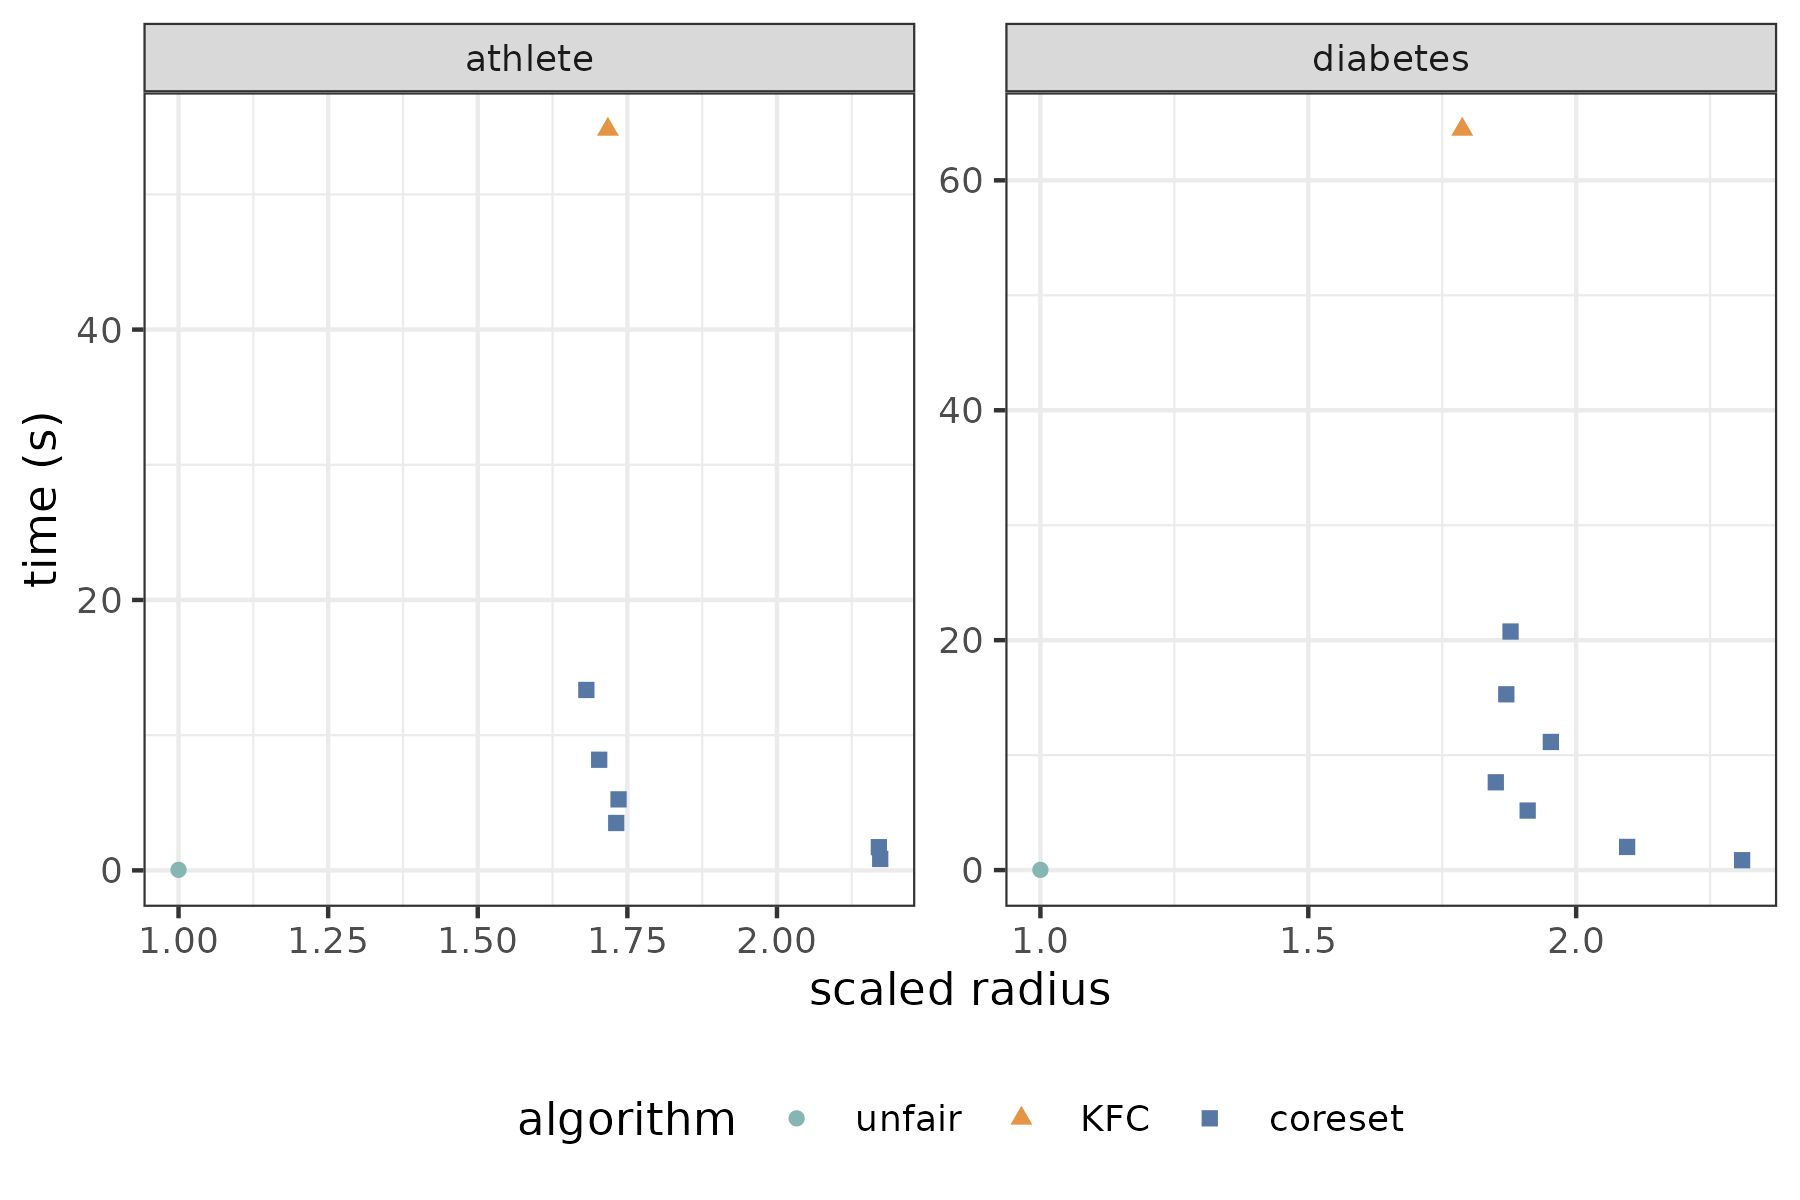
\includegraphics[width=\textwidth]{figs/time-vs-radius-k32-small.png}
	\texttt{athlete} 206k points,
	\texttt{diabetes} 90k points
\end{frame}

\begin{frame}{Experiments}
	\centering
	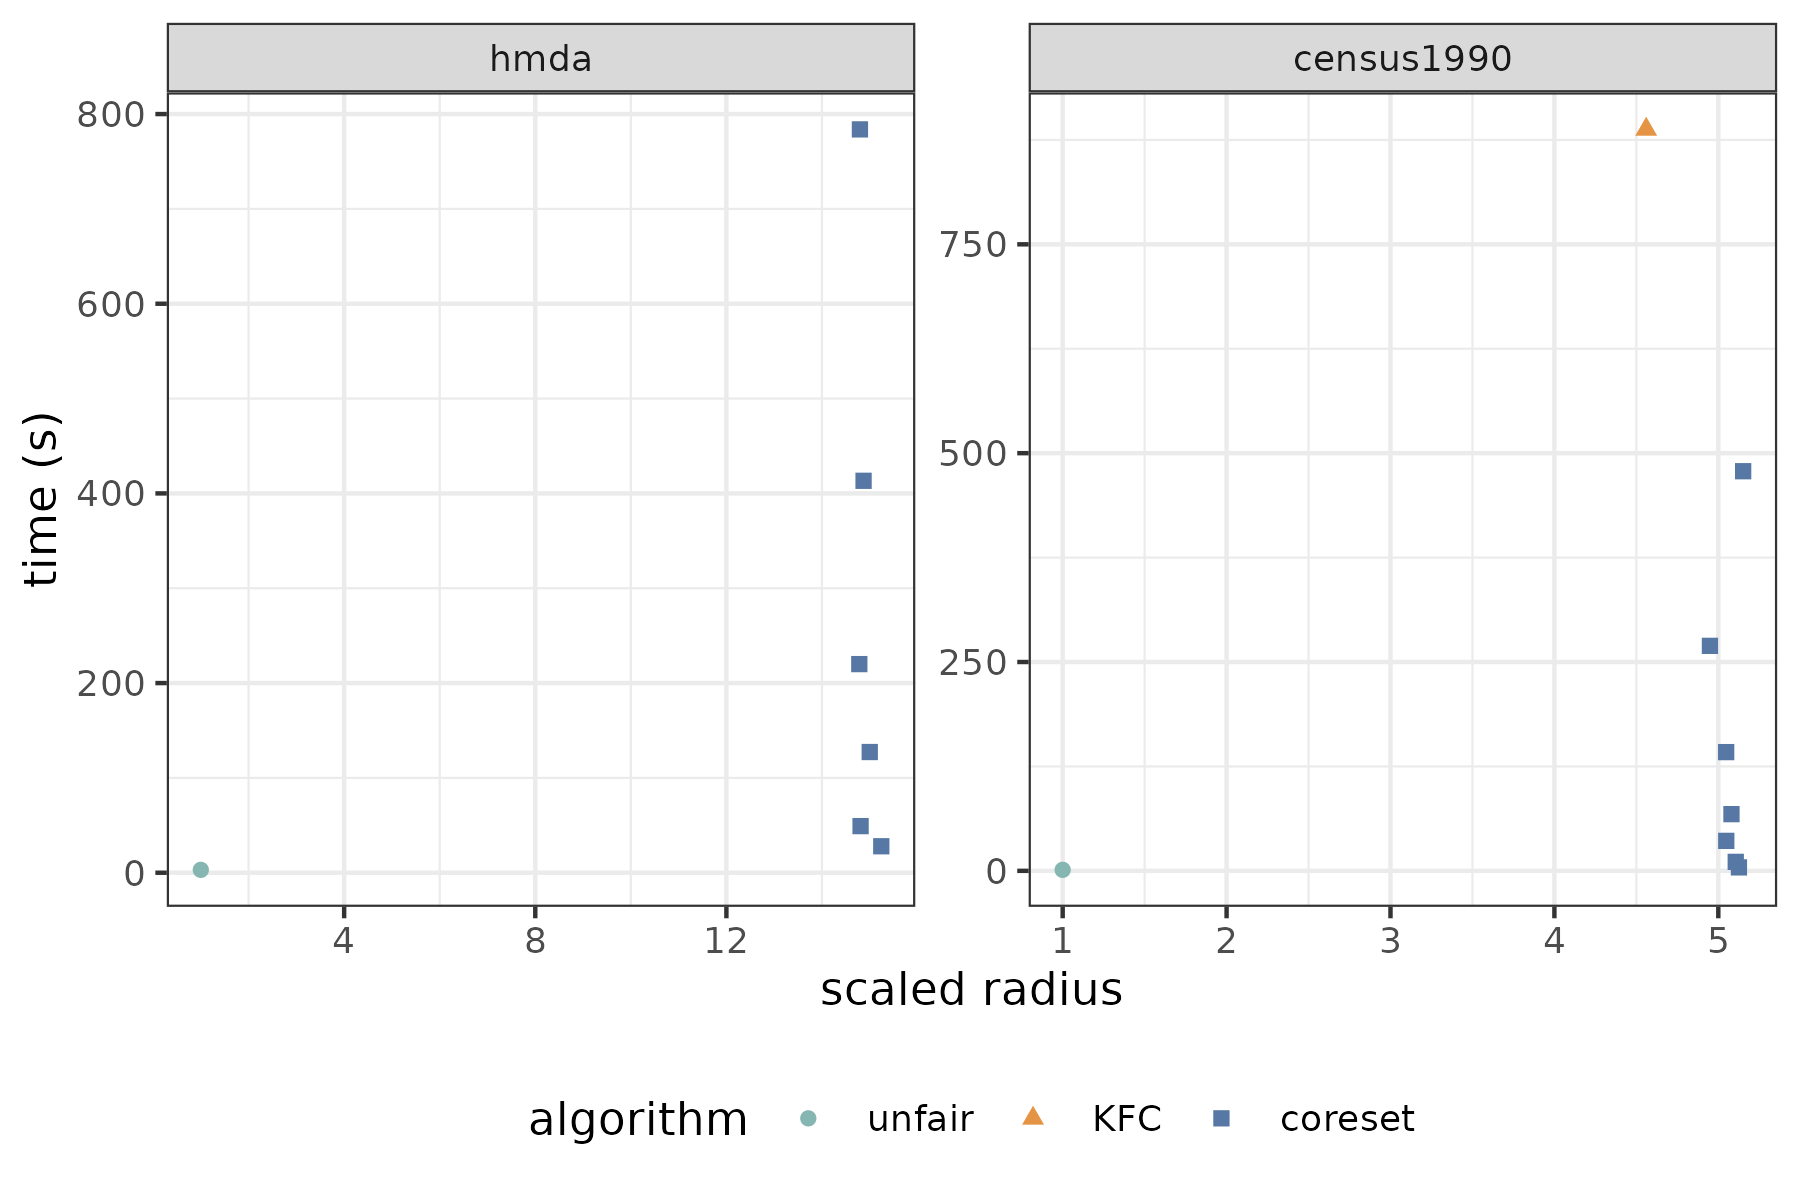
\includegraphics[width=\textwidth]{figs/time-vs-radius-k32-larger.png}
	\texttt{hmda} 16M points,
	\texttt{census1990} 2.5M points
\end{frame}





\begin{frame}{Conclusions}
	\begin{block}{So what?}
		\begin{itemize}
			\item We have $3+\epsilon$ approximation algorithm that scales to large data
			\item Also in MapReduce and Streaming (insertion only)
			\item With a practical implementation (with a linear programming solver for the solution)
		\end{itemize}
	\end{block}

	\pause

	\begin{block}{And now?}
		\begin{itemize}
			\item Finish writing the paper \emoji{grinning-face-with-sweat}
			\item Outliers?
			\item Purely combinatorial algorithms?
		\end{itemize}
	\end{block}
\end{frame}







\end{document}

